\setcounter{framenumber}{0}
%45

\begin{frame}
  \titlepage
\end{frame}

\begin{frame}{Learning Goals}
By the end of this lecture, students should be able to:
\begin{itemize}
    \item define joint, marginal, and conditional distributions;
    \item understand independence of random variables;
    \item apply the two-dimensional LOTUS formula;
    \item define covariance and correlation;
    \item distinguish independence from zero correlation;
    \item define pairwise and mutual independence;
    \item define the Multinomial distribution;
    \item understand the Multivariate Normal distribution.
\end{itemize}
\end{frame}

\lecturepart{Joint Distributions}

\begin{frame}{Why Joint Distributions?}
Previously, we studied one random variable at a time.

\vspace{0.25cm}

But many probabilistic questions involve several random variables simultaneously.

\vspace{0.25cm}

Examples:
\begin{itemize}
    \item height and weight;
    \item temperature and rainfall;
    \item several coin tosses;
    \item sums of random variables;
    \item sample means.
\end{itemize}

\vspace{0.25cm}

\begin{keybox}{Main idea}
Joint distributions describe how multiple random variables behave together.
\end{keybox}
\end{frame}

\begin{frame}{Joint PMF}
\begin{keybox}{Definition}
For discrete random variables \(X,Y\), the joint PMF is
\[
p_{X,Y}(x,y)
=
\Prob(X=x,Y=y).
\]
\end{keybox}

Properties:
\[
p_{X,Y}(x,y)\ge0, \quad and \quad \sum_x\sum_y p_{X,Y}(x,y)=1.
\]
\vspace{2mm}
\hrule
\vspace{2mm}
Similarly, for $n$ discrete random variables $X_1,\dots, X_n$, the joint PMF is
\begin{equation*}
    p_{X_1,\dots, X_n}(x_1,\dots, x_n)= \mathbb{P}(X_1=x_1, \dots ,X_n=x_n)
\end{equation*}
\textbf{Note} $\{X\leq x, Y\leq y\} = \{X\leq x\} \cap \{Y\leq y\}$

\end{frame}



\begin{frame}{Marginal PMFs}

\textbf{Question} How to find $p_X(x)$ (the PMF of $X$) and $p_Y(y)$ (the PMF of $Y$) using $p_{X,Y}(x,y)$ (the joint distribution of $X$ and $Y$)?
\vspace{1mm}
\\
\textbf{Answer: }The marginal PMFs are obtained by summing out the other variable.

\vspace{0.25cm}

\[
{
p_X(x)
=
\sum_y p_{X,Y}(x,y)
}
\]

and

\[
{
p_Y(y)
=
\sum_x p_{X,Y}(x,y).
}
\]

\begin{keybox}{Remark}
Marginal's distribution can be obtained via (summing up) the joint distribution but not necessarily vice versa. We will see that independence enables us to also find the joint distribution through the marginal distributions.
\end{keybox}
 
\end{frame}




 











\begin{frame}{Example: Two Fair Dice and Marginals}
Let $X$ be the outcome of the first die and $Y$ the outcome of the second die.

\[
p_{X,Y}(x,y)=\Prob(X=x,Y=y)=\frac1{36},
\qquad x,y\in\{1,2,3,4,5,6\}.
\]

\[
\renewcommand{\arraystretch}{1.25}
\begin{array}{c|cccccc|c}
p_{X,Y}(x,y) =\Prob(X=x, Y=y)& y=1 & y=2 & y=3 & y=4 & y=5 & y=6 & p_X(x)=\Prob(X=x)\\
\hline
x=1 & \frac1{36} & \frac1{36} & \frac1{36} & \frac1{36} & \frac1{36} & \frac1{36} & \frac6{36}\\
x=2 & \frac1{36} & \frac1{36} & \frac1{36} & \frac1{36} & \frac1{36} & \frac1{36} & \frac6{36}\\
x=3 & \frac1{36} & \frac1{36} & \frac1{36} & \frac1{36} & \frac1{36} & \frac1{36} & \frac6{36}\\
x=4 & \frac1{36} & \frac1{36} & \frac1{36} & \frac1{36} & \frac1{36} & \frac1{36} & \frac6{36}\\
x=5 & \frac1{36} & \frac1{36} & \frac1{36} & \frac1{36} & \frac1{36} & \frac1{36} & \frac6{36}\\
x=6 & \frac1{36} & \frac1{36} & \frac1{36} & \frac1{36} & \frac1{36} & \frac1{36} & \frac6{36}\\
\hline
p_Y(y)=\Prob(Y=y) & \frac6{36} & \frac6{36} & \frac6{36} & \frac6{36} & \frac6{36} & \frac6{36} &
\end{array}
\]
For example,
\[
p_X(3)=\sum_{y=1}^6 p_{X,Y}(3,y)
=
\frac1{36}+\cdots+\frac1{36}
=
\frac6{36}
=
\frac16, \quad and\quad p_Y(4)=\sum_{x=1}^6 p_{X,Y}(x,4)
=
\frac6{36}
=
\frac16.
\]
The marginal PMFs appear on the "margins" of the joint PMF table.
\end{frame}














\begin{frame}{Proof of Marginal PMFs}
We prove the formula for $p_X(x)$.


Fix a value $x$ in the support of $X$. Then
\[
p_X(x)
=
\Prob(X=x).
\]

The event $\{X=x\}$ can be written as the union of all events
\[
\{X=x,\;Y=y\}
\]
over all possible values $y$ of $Y$:

\[
\{X=x\}
=
\bigcup_y \{X=x,\;Y=y\}.
\]
Reason:
\begin{equation*}
    \{X = x \} = \big ( \{X=x\} \cap\Sample \big )= \{ X=x\} \cap ( \bigcup_{y}\{ Y=y\}) =  \bigcup_y \{ X=x\}\cap \{Y=y \}  =  \bigcup_y \{X=x, Y=y \}
\end{equation*}
Thus, applying the probability function to the above equation yields the result. Indeed, these events are pairwise disjoint, because $Y$ cannot take two different
values at the same time. Therefore, by the third axiom of probability (countable additivity),

\[
\Prob(X=x)
=
\sum_y \Prob(X=x,\;Y=y).
\]

Hence,

\[
\boxed{
p_X(x)
=
\sum_y p_{X,Y}(x,y).
}
\]

The proof for $p_Y(y)$ is identical:

\[
\boxed{
p_Y(y)
=
\sum_x p_{X,Y}(x,y).
}
\]
\end{frame}











\begin{frame}{Conditional PMFs}
\begin{keybox}{Definition}
If
\[
\Prob(X=x)>0,
\]
then
\[
{
p_{Y|X}(y|x)
=
\Prob(Y=y|X=x)
=
\frac{
p_{X,Y}(x,y)
}{
p_X(x)
}.
}
\]
\end{keybox}

\vspace{0.25cm}

Conditional distributions describe one variable given information about another.
\end{frame}
\begin{frame}{Joint PDFs}
\begin{keybox}{Definition}
For continuous random variables \(X,Y\), the joint PDF is a function
\[
f_{X,Y}(x,y)
\]
such that
\[
\Prob((X,Y)\in A)
=
\iint_A f_{X,Y}(x,y)\,dx\,dy.
\]
\end{keybox}

 

Properties:
\[
f_{X,Y}(x,y)\ge0,
\qquad
\iint_{\mathbb{R}^2} f_{X,Y}(x,y)\,dx\,dy=1.
\]

 

Similarly, for $n$ continuous random variables
\[
X_1,\dots,X_n,
\]
the joint PDF is a function
\[
f_{X_1,\dots,X_n}(x_1,\dots,x_n)
\]
such that
\[
\mathbb{P}\big((X_1,\dots,X_n)\in A\big)
=
\int_A \cdots \int
f_{X_1,\dots,X_n}(x_1,\dots,x_n)
\,dx_1\cdots dx_n.
\]
\end{frame}


\begin{frame}{Marginal PDFs}
Marginal densities are obtained by integrating out the other variable.

\vspace{0.25cm}

\[
{
f_X(x)
=
\int_{-\infty}^\infty
f_{X,Y}(x,y)\,dy
}
\]

and

\[
{
f_Y(y)
=
\int_{-\infty}^\infty
f_{X,Y}(x,y)\,dx.
}
\]
\end{frame}

\begin{frame}{Conditional PDFs}
\begin{keybox}{Definition}
If
\[
f_X(x)>0,
\]
then
\[
{
f_{Y|X}(y|x)
=
\frac{
f_{X,Y}(x,y)
}{
f_X(x)
}.
}
\]
\end{keybox}
\end{frame}

















% =====================================================
% JOINT CDFS
% Insert after Conditional PMFs and before Joint PDFs
% =====================================================

\begin{frame}{Joint Cumulative Distribution Function}

\begin{keybox}{Definition: Two Random Variables}
For any two random variables \(X\) and \(Y\), their joint cumulative
distribution function, or joint CDF, is
\[
\boxed{
F_{X,Y}(x,y)
=
\Prob(X\le x,\;Y\le y),
\qquad (x,y)\in\mathbb{R}^2.
}
\]
\end{keybox}

Since
\[
\{X\le x,\;Y\le y\}
=
\{X\le x\}\cap\{Y\le y\},
\]
we may equivalently write
\[
F_{X,Y}(x,y)
=
\Prob\big(\{X\le x\}\cap\{Y\le y\}\big).
\]

\vspace{0.2cm}

Geometrically,
\[
F_{X,Y}(x,y)
\]
is the probability that the random point \((X,Y)\) lies in the
southwest rectangle
\[
(-\infty,x]\times(-\infty,y].
\]

\begin{keybox}{Important}
The joint CDF is defined for every pair of random variables:
discrete, continuous, or mixed.
\end{keybox}

\end{frame}








\begin{frame}{Joint CDF of \(n\) Random Variables}

Let
\[
\mathbf{X}
=
(X_1,\dots,X_n)
\]
be an \(n\)-dimensional random vector.

\begin{keybox}{Definition}
The joint CDF of \(X_1,\dots,X_n\) is
\[
\boxed{
F_{X_1,\dots,X_n}(x_1,\dots,x_n)
=
\Prob(X_1\le x_1,\dots,X_n\le x_n).
}
\]
\end{keybox}

Equivalently,
\[
F_{\mathbf X}(\mathbf x)
=
\Prob\left(
\bigcap_{i=1}^{n}\{X_i\le x_i\}
\right).
\]

Geometrically, it gives the probability that
\[
(X_1,\dots,X_n)
\]
belongs to the lower-left \(n\)-dimensional rectangle
\[
(-\infty,x_1]\times\cdots\times(-\infty,x_n].
\]

When \(n=1\), this reduces to the ordinary CDF:
\[
F_X(x)=\Prob(X\le x).
\]

\end{frame}













\begin{frame}{Basic Properties of a Joint CDF}

For every \(x,y\in\mathbb{R}\),

\begin{enumerate}
    \item \textbf{Bounds:}
    \[
    \boxed{
    0\le F_{X,Y}(x,y)\le 1.
    }
    \]

    \item \textbf{Nondecreasing in each coordinate:}

    If \(x_1\le x_2\), then
    \[
    F_{X,Y}(x_1,y)
    \le
    F_{X,Y}(x_2,y).
    \]

    If \(y_1\le y_2\), then
    \[
    F_{X,Y}(x,y_1)
    \le
    F_{X,Y}(x,y_2).
    \]

    \item \textbf{Right-continuity:}

    If
    \[
    x_m\downarrow x
    \qquad\text{and}\qquad
    y_m\downarrow y,
    \]
    then
    \[
    \boxed{
    F_{X,Y}(x_m,y_m)
    \longrightarrow
    F_{X,Y}(x,y).
    }
    \]
\end{enumerate}

\begin{keybox}{Interpretation}
Increasing either threshold enlarges the event whose probability is
being calculated, so the joint CDF cannot decrease.
\end{keybox}

\end{frame}





\begin{frame}{Limits of a Joint CDF}

The joint CDF satisfies the following boundary conditions.

If either coordinate approaches \(-\infty\), then
\[
\boxed{
\lim_{x\to-\infty}F_{X,Y}(x,y)=0
}
\]
for every fixed \(y\), and
\[
\boxed{
\lim_{y\to-\infty}F_{X,Y}(x,y)=0
}
\]
for every fixed \(x\).

If both coordinates approach \(+\infty\), then
\[
\boxed{
\lim_{\substack{x\to\infty\\y\to\infty}}
F_{X,Y}(x,y)
=
1.
}
\]

Indeed,
\[
\{X\le x,\;Y\le y\}
\uparrow
\Sample
\]
as \(x,y\to\infty\), so
\[
\Prob(X\le x,\;Y\le y)\longrightarrow\Prob(\Sample)=1.
\]

\end{frame}


\begin{frame}{Obtaining Marginal CDFs from the Joint CDF}

The marginal CDFs can be obtained by sending the other threshold to
\(+\infty\).

\begin{keybox}{Marginal CDFs}
\[
\boxed{
F_X(x)
=
\lim_{y\to\infty}F_{X,Y}(x,y)
}
\]
and
\[
\boxed{
F_Y(y)
=
\lim_{x\to\infty}F_{X,Y}(x,y).
}
\]
\end{keybox}

For example,
\[
\begin{aligned}
\lim_{y\to\infty}F_{X,Y}(x,y)
&=
\lim_{y\to\infty}
\Prob(X\le x,\;Y\le y)
\\
&=
\Prob(X\le x)
\\
&=
F_X(x).
\end{aligned}
\]

This works because
\[
\{Y\le y\}\uparrow\Sample
\qquad\text{as }y\to\infty.
\]

Similarly,
\[
\lim_{x\to\infty}F_{X,Y}(x,y)=F_Y(y).
\]

\end{frame}




\begin{frame}{Marginal CDFs in \(n\) Dimensions}

Suppose
\[
F_{X_1,\dots,X_n}(x_1,\dots,x_n)
\]
is known.

To obtain the CDF of \(X_i\), send every other coordinate to
\(+\infty\):

\[
\boxed{
F_{X_i}(x_i)
=
\lim_{\substack{x_j\to\infty\\j\neq i}}
F_{X_1,\dots,X_n}(x_1,\dots,x_n).
}
\]

More generally, let
\[
I=\{i_1,\dots,i_k\}
\subseteq
\{1,\dots,n\}.
\]

The joint CDF of the subvector
\[
(X_{i_1},\dots,X_{i_k})
\]
is
\[
\boxed{
F_{X_{i_1},\dots,X_{i_k}}
(x_{i_1},\dots,x_{i_k})
=
\lim_{\substack{x_j\to\infty\\j\notin I}}
F_{X_1,\dots,X_n}(x_1,\dots,x_n).
}
\]

Thus every lower-dimensional marginal CDF can be derived from the
full joint CDF.

\end{frame}














\begin{frame}{Properties of an \(n\)-Dimensional Joint CDF}

The joint CDF
\[
F_{X_1,\dots,X_n}(x_1,\dots,x_n)
\]
has the following properties:

\begin{enumerate}
    \item
    \[
    0\le F_{X_1,\dots,X_n}(x_1,\dots,x_n)\le1.
    \]

    \item It is nondecreasing in each coordinate.

    \item It is right-continuous in each coordinate.

    \item If any one coordinate tends to \(-\infty\), then
    \[
    F_{X_1,\dots,X_n}(x_1,\dots,x_n)\longrightarrow0.
    \]

    \item If every coordinate tends to \(+\infty\), then
    \[
    F_{X_1,\dots,X_n}(x_1,\dots,x_n)\longrightarrow1.
    \]

    \item It assigns nonnegative probability to every
    \(n\)-dimensional rectangle.
\end{enumerate}

The final property is called the
\[
\boxed{\text{\(n\)-increasing property.}}
\]

\end{frame}




\begin{frame}{From the Joint CDF to a Joint PDF}

Every random vector has a joint CDF, but not every random vector has
a joint PDF.

\vspace{0.2cm}

If \(X\) and \(Y\) have a joint PDF \(f_{X,Y}\), then
\[
\boxed{
F_{X,Y}(x,y)
=
\int_{-\infty}^{x}
\int_{-\infty}^{y}
f_{X,Y}(u,v)\,dv\,du.
}
\]

Thus the joint CDF accumulates the density over the southwest
rectangle
\[
(-\infty,x]\times(-\infty,y].
\]

If \(F_{X,Y}\) is sufficiently differentiable, then
\[
\boxed{
f_{X,Y}(x,y)
=
\frac{\partial^2}{\partial x\,\partial y}
F_{X,Y}(x,y).
}
\]

\begin{keybox}{Connection}
The PDF is obtained by differentiating the CDF, while the CDF is
obtained by integrating the PDF.
\end{keybox}

\end{frame}












%=========================================================
\begin{frame}{Probabilities of Rectangles from the Joint CDF}

Let
$$
a_1<a_2
\qquad\text{and}\qquad
b_1<b_2.
$$

For the rectangle
$$
a_1<X\le a_2,
\qquad
b_1<Y\le b_2,
$$
we have
$$
\boxed{
\begin{aligned}
&\Prob(a_1<X\le a_2,\;b_1<Y\le b_2)
\\[1mm]
&\qquad =
F_{X,Y}(a_2,b_2)
-
F_{X,Y}(a_1,b_2)
-
F_{X,Y}(a_2,b_1)
+
F_{X,Y}(a_1,b_1).
\end{aligned}
}
$$

This is the two-dimensional inclusion--exclusion formula.
 

\end{frame}




\begin{frame}{Visualizing the Joint CDF}

\begin{center}
    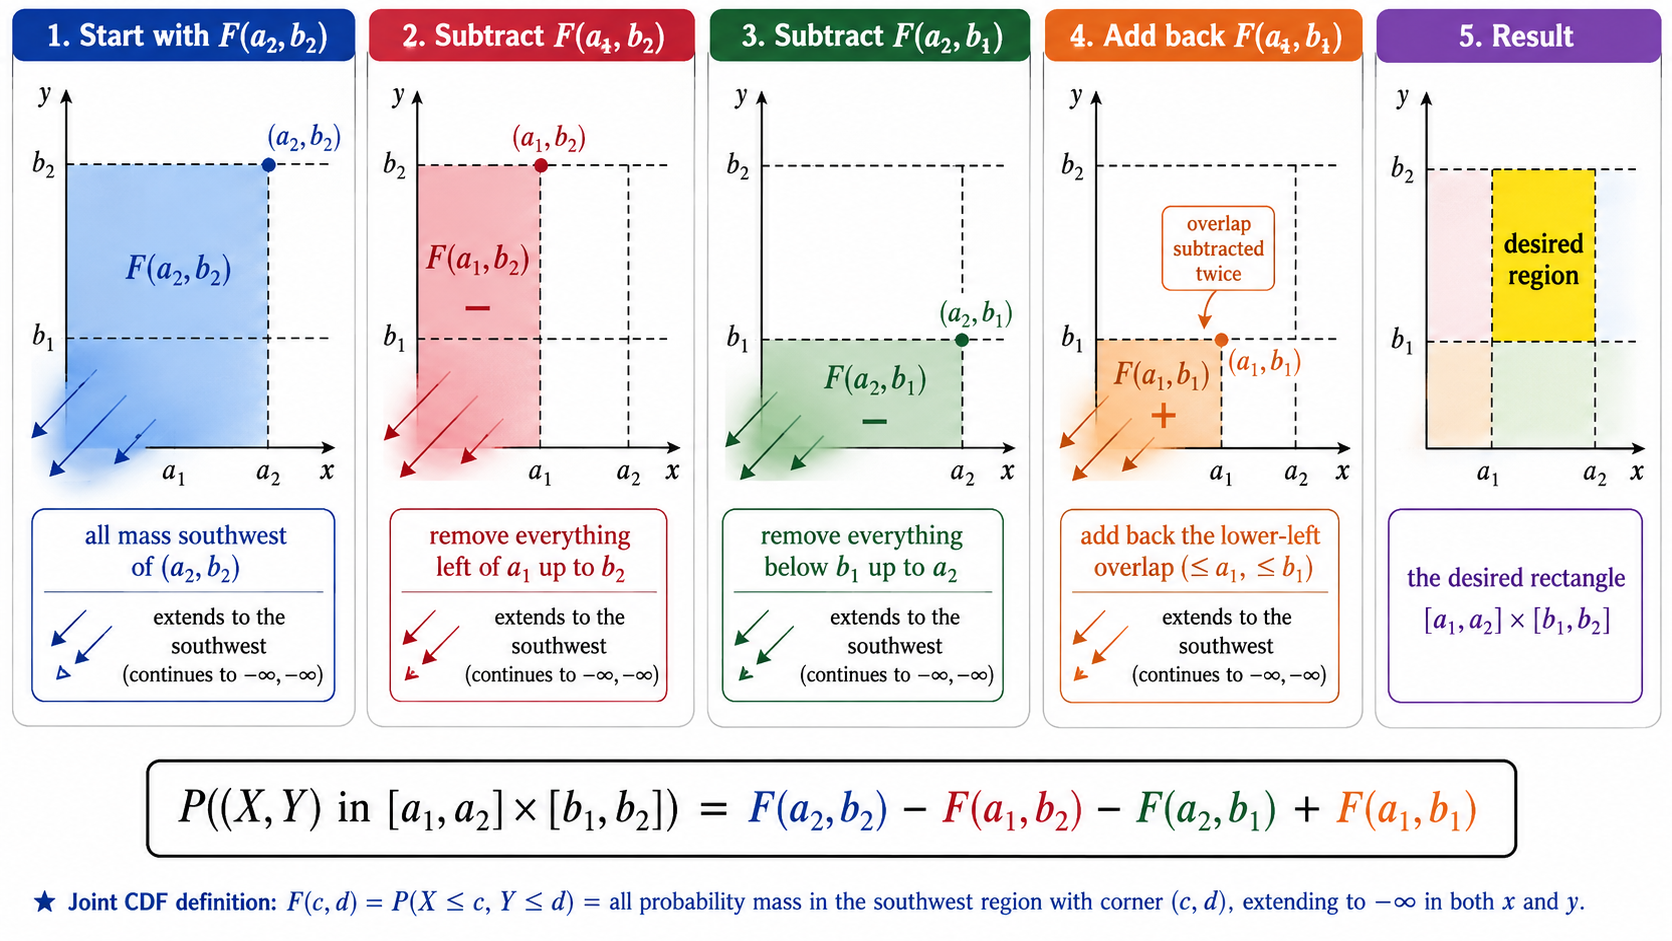
\includegraphics[width=0.9\textwidth]{assets/figures/joint-cdf-corner.png}
\end{center}

\end{frame}




%=========================================================
\begin{frame}{Joint CDF: One Bounded Interval and One One-Sided Interval}

Recall that the marginal CDFs can be recovered from the joint CDF:
$$
F_X(x)
=
\lim_{y\to\infty}F_{X,Y}(x,y),
\qquad
F_Y(y)
=
\lim_{x\to\infty}F_{X,Y}(x,y).
$$

\textbf{Bounded in $X$, one-sided in $Y$:}

$$
\boxed{
\Prob(a_1<X\le a_2,\;Y\le b_2)
=
F_{X,Y}(a_2,b_2)-F_{X,Y}(a_1,b_2)
}
$$

$$
\boxed{
\begin{aligned}
\Prob(a_1<X\le a_2,\;Y>b_1)
&=
F_X(a_2)-F_X(a_1)
\\
&\quad
-F_{X,Y}(a_2,b_1)
+F_{X,Y}(a_1,b_1).
\end{aligned}
}
$$

\textbf{One-sided in $X$, bounded in $Y$:}

$$
\boxed{
\Prob(X\le a_2,\;b_1<Y\le b_2)
=
F_{X,Y}(a_2,b_2)-F_{X,Y}(a_2,b_1)
}
$$

$$
\boxed{
\begin{aligned}
\Prob(X>a_1,\;b_1<Y\le b_2)
&=
F_Y(b_2)-F_Y(b_1)
\\
&\quad
-F_{X,Y}(a_1,b_2)
+F_{X,Y}(a_1,b_1).
\end{aligned}
}
$$

\end{frame}


%=========================================================
\begin{frame}{Joint CDF: When Both Conditions Are One-Sided}

There are four possible combinations.

\vspace{0.15cm}

\textbf{Both are lower-tail events:}
$$
\boxed{
\Prob(X\le a_2,\;Y\le b_2)
=
F_{X,Y}(a_2,b_2)
}
$$

\textbf{$X$ upper-tail, $Y$ lower-tail:}
$$
\boxed{
\Prob(X>a_1,\;Y\le b_2)
=
F_Y(b_2)-F_{X,Y}(a_1,b_2)
}
$$

\textbf{$X$ lower-tail, $Y$ upper-tail:}
$$
\boxed{
\Prob(X\le a_2,\;Y>b_1)
=
F_X(a_2)-F_{X,Y}(a_2,b_1)
}
$$

\textbf{Both are upper-tail events:}
$$
\boxed{
\begin{aligned}
\Prob(X>a_1,\;Y>b_1)
&=
1-F_X(a_1)-F_Y(b_1)
\\
&\quad
+F_{X,Y}(a_1,b_1).
\end{aligned}
}
$$

\end{frame}

 





\begin{frame}{Deriving the Rectangle Formula}

Let
$$
a_1<a_2,
\qquad
b_1<b_2,
$$
and consider the event
$$
R=\{a_1<X\le a_2,\;b_1<Y\le b_2\}.
$$

Define
$$
E=\{X\le a_2,\;Y\le b_2\},
$$
the large southwest region ending at $(a_2,b_2)$.

Inside $E$, the points we do \emph{not} want are
$$
L=\{X\le a_1,\;Y\le b_2\},
\qquad
B=\{X\le a_2,\;Y\le b_1\}.
$$

Hence, as an equality of events,
$$
\boxed{
R=E\setminus(L\cup B).
}
$$

Therefore,
$$
\begin{aligned}
\Prob(R)
&=\Prob(E)-\Prob(L\cup B)\\
&=\Prob(E)-\Prob(L)-\Prob(B)+\Prob(L\cap B),
\end{aligned}
$$
where the second equality follows from inclusion--exclusion.


\end{frame}



\begin{frame}{Continue.}
    
Now,
$$
L\cap B
=
\{X\le a_1,\;Y\le b_1\}.
$$
Using
$$
F_{X,Y}(x,y)=\Prob(X\le x,\;Y\le y),
$$
we obtain
$$
\begin{aligned}
\Prob(a_1<X\le a_2,\;b_1<Y\le b_2)
&=
F_{X,Y}(a_2,b_2)
-
F_{X,Y}(a_1,b_2)
\\
&\quad
-
F_{X,Y}(a_2,b_1)
+
F_{X,Y}(a_1,b_1).
\end{aligned}
$$

\begin{keybox}{Rectangle probability from the joint CDF}
$$
\boxed{
\Prob(a_1<X\le a_2,\;b_1<Y\le b_2)
=
F_{X,Y}(a_2,b_2)
-
F_{X,Y}(a_1,b_2)
-
F_{X,Y}(a_2,b_1)
+
F_{X,Y}(a_1,b_1).
}
$$
\end{keybox}

\end{frame}





 








 







%=========================================================
\begin{frame}{Example}

Suppose $(X,Y)$ has joint PDF
$$
f_{X,Y}(x,y)
=
\begin{cases}
2, & 0<y<x<1,\\
0, & \text{otherwise}.
\end{cases}
$$
 

\textbf{PDF verification}:

Since $f_{X,Y}(x,y) \in \{ 0,2 \}$,
we only need to check that it integrates to $1$:

 
\begin{equation}
\int_{-\infty}^{\infty}
\int_{-\infty}^{\infty}
f_{X,Y}(x,y)\,dy\,dx
=
\int_0^1\int_0^x 2\,dy\,dx
=
\int_0^1 2x\,dx
=
\left[x^2\right]_0^1
=1.
\end{equation}
 

Therefore $f_{X,Y}$ is a valid joint density.

\begin{keybox}{Important}
The inequalities defining the support determine the limits of integration:
$$
0<x<1,
\qquad
0<y<x.
$$
\end{keybox}

\end{frame}


%=========================================================
\begin{frame}{Deriving the Marginal Densities}

To obtain the marginal density of $X$, integrate out $Y$:

$$
f_X(x)
=
\int_{-\infty}^{\infty}
f_{X,Y}(x,y)\,dy.
$$

For a fixed $x$ with $0<x<1$, the support requires $0<y<x.$ Therefore,
 
\begin{equation}
f_X(x)
=
\int_0^x 2\,dy = 2x.
\end{equation}
 

Hence,
$$
{
f_X(x)
=
\begin{cases}
2x, & 0<x<1,\\
0, & \text{otherwise}.
\end{cases}
}
$$

Similarly, to obtain the marginal density of $Y$, integrate out $X$:

$$
f_Y(y)
=
\int_{-\infty}^{\infty}
f_{X,Y}(x,y)\,dx.
$$

For a fixed $y$ with $0<y<1$, the support condition $y<x<1$ gives

$$
{
f_Y(y)
=
\begin{cases}
2(1-y), & 0<y<1,\\
0, & \text{otherwise}.
\end{cases}
}
$$
\end{frame}


%=========================================================
\begin{frame}{Checking the Marginals}

Each marginal density must itself integrate to $1$.

For $X$,
\[
\int_0^1 f_X(x)\,dx
=
\int_0^1 2x\,dx
=
\left[x^2\right]_0^1
=
1.
\]

For $Y$,
\[
\int_0^1 f_Y(y)\,dy
=
\int_0^1 2(1-y)\,dy
=
\left[2y-y^2\right]_0^1
=
1.
\]

Therefore,
\[
\boxed{
\int_{-\infty}^{\infty} f_X(x)\,dx
=
\int_{-\infty}^{\infty} f_Y(y)\,dy
=
1
}
\]

Thus, both $f_X$ and $f_Y$ are valid marginal probability density functions.

\end{frame}


%=========================================================
\begin{frame}{Deriving the Joint CDF from the Joint PDF}

Recall the definition:
$$
F_{X,Y}(x,y)
=
\Prob(X\le x,\;Y\le y).
$$

For continuous random variables,
$$
\boxed{
F_{X,Y}(x,y)
=
\int_{-\infty}^{x}
\int_{-\infty}^{y}
f_{X,Y}(u,v)\,dv\,du.
}
$$

However, the limits must respect the support
$$
0<v<u<1.
$$

Consequently, the calculation depends on the location of $(x,y)$.

\textbf{Case 1: $x\le0$ or $y\le0$.}

There is no probability mass southwest of $(x,y)$, so
$$
{F_{X,Y}(x,y)=0.}
$$

\textbf{Case 2: $0<x\le1$ and $y\ge x$.}

Since every supported point with $X\le x$ automatically satisfies
$Y<X\le x\le y$,

\begin{equation}
F_{X,Y}(x,y)=
\int_0^x\int_0^u 2\,dv\,du = \int_0^x 2u\,du =
x^2.
\end{equation}
 
Thus, ${F_{X,Y}(x,y)=x^2.}$
 
\end{frame}


%=========================================================
\begin{frame}{Deriving the Joint CDF: The Nontrivial Case}

Now suppose
$$
0<y<x\le1.
$$

The restriction $Y\le y$ cuts through the support, so the integral
must be split at $u=y$:

$$
\begin{aligned}
F_{X,Y}(x,y)
&=
\int_0^y\int_0^u 2\,dv\,du
+
\int_y^x\int_0^y 2\,dv\,du.
\end{aligned}
$$

The first term gives
$$
\int_0^y 2u\,du
=
y^2,
$$

while the second gives
$$
\int_y^x 2y\,du
=
2y(x-y).
$$

Therefore,
$$
\begin{aligned}
F_{X,Y}(x,y)
&=
y^2+2y(x-y)\\
&=
2xy-y^2.
\end{aligned}
$$

Hence,
$$
{
F_{X,Y}(x,y)=2xy-y^2,
\qquad
0<y<x\le1.
}
$$


\end{frame}


%=========================================================
\begin{frame}{The Complete Joint CDF}

Combining all cases gives

$$
\boxed{
F_{X,Y}(x,y)
=
\begin{cases}
0,
& x\le0 \text{ or } y\le0,
\\[2mm]
x^2,
& 0<x\le1,\quad y\ge x,
\\[2mm]
2xy-y^2,
& 0<y<x\le1,
\\[2mm]
2y-y^2,
& x\ge1,\quad 0<y<1,
\\[2mm]
1,
& x\ge1,\quad y\ge1.
\end{cases}
}
$$

The term
$$
2y-y^2
$$
for $x\ge1$ arises because once $x\ge1$, the condition $X\le x$
places no further restriction on the support:

$$
F_{X,Y}(x,y)
=
\Prob(Y\le y)
=
F_Y(y).
$$

Similarly, whenever $y\ge1$,
$$
F_{X,Y}(x,y)
=
\Prob(X\le x)
=
F_X(x).
$$

\end{frame}


%=========================================================
\begin{frame}{Recovering the PDF from the Joint CDF}

For an absolutely continuous random vector,

$$
{
f_{X,Y}(x,y)
=
\frac{\partial^2}{\partial x\,\partial y}
F_{X,Y}(x,y)
}
$$

at points where the derivatives exist.

Inside the support, $0<y<x<1,$ we found
$$
F_{X,Y}(x,y)
=
2xy-y^2.
$$

Differentiate first with respect to $y$:

$$
\frac{\partial}{\partial y}F_{X,Y}(x,y)
=
2x-2y.
$$

Then differentiate with respect to $x$:

$$
\frac{\partial}{\partial x}
\left(2x-2y\right)
=
2.
$$

Therefore,
$$
{
\frac{\partial^2}{\partial x\,\partial y}
F_{X,Y}(x,y)
=
2
=
f_{X,Y}(x,y),
\qquad 0<y<x<1.
}
$$

Outside the support, the mixed derivative is $0$ wherever it exists,
which again agrees with the joint density.

\end{frame}


%=========================================================
\begin{frame}{Recovering the Marginal CDFs from the Joint CDF}

For any joint CDF,

$$
{
F_X(x)
=
\lim_{y\to\infty}F_{X,Y}(x,y)
}
$$
For this example,

$$
F_X(x)
=
\begin{cases}
0, & x\le0,\\
x^2, & 0<x<1,\\
1, & x\ge1.
\end{cases}
$$

Indeed,
$$
F_X(x)
=
\int_{-\infty}^x f_X(u)\,du
=
\int_0^x 2u\,du
=
x^2,
\qquad 0<x<1.
$$

Similarly,
$$
F_Y(y)
=
\begin{cases}
0, & y\le0,\\
2y-y^2, & 0<y<1,\\
1, & y\ge1.
\end{cases}
$$

since
$
F_Y(y)
=
\int_0^y 2(1-v)\,dv
=
2y-y^2.
$

\end{frame}

 




\begin{frame}{Example: Uniform on the Unit Disk}
Suppose \((X,Y)\) is uniformly distributed on the unit disk
\[
D=\{(x,y):x^2+y^2\le 1\}.
\]

Since the area of the unit disk is \(\pi\), the joint density is
\[
f_{X,Y}(x,y)
=
\begin{cases}
\dfrac{1}{\pi}, & x^2+y^2\le 1,\\[6pt]
0, & \text{otherwise}.
\end{cases}
\]

Indeed,
\[
\iint_{\mathbb{R}^2} f_{X,Y}(x,y)\,dx\,dy
=
\iint_D \frac{1}{\pi}\,dx\,dy
=
\frac{1}{\pi}\operatorname{Area}(D)
=
1.
\]

For a fixed value of \(X=x\), the possible values of \(Y\) satisfy
\[
-\sqrt{1-x^2}\le Y\le \sqrt{1-x^2}.
\]

\begin{keybox}{Important}
Knowing \(X\) restricts the possible values of \(Y\), so \(X\) and \(Y\) are dependent.
\end{keybox}
\end{frame}


















\begin{frame}{Multivariate Moment Generating Function}

Let
$$
\mathbf X=(X_1,\dots,X_n)^\top
$$
be a random vector. Its \textbf{joint moment generating function (MGF)} is defined by
$$
\boxed{
M_{\mathbf X}(\mathbf t)
=
\E\!\left[e^{\mathbf t^\top \mathbf X}\right]
=
\E\!\left[
e^{t_1X_1+\cdots+t_nX_n}
\right],
}
$$
for all
$$
\mathbf t=(t_1,\dots,t_n)^\top
$$
for which the expectation is finite.

In the two-dimensional case,
$$
\boxed{
M_{X,Y}(s,t)
=
\E\!\left[e^{sX+tY}\right].
}
$$
 
 

\end{frame}



%=========================================================
\begin{frame}{Multivariate Moment Generating Function}

Let
$$
\mathbf X=(X_1,\dots,X_n)^\top
$$
be a random vector. Its \textbf{joint moment generating function (MGF)} is defined by
$$
\boxed{
M_{\mathbf X}(\mathbf t)
=
\E\!\left[e^{\mathbf t^\top \mathbf X}\right]
=
\E\!\left[
e^{t_1X_1+\cdots+t_nX_n}
\right],
}
$$
for all
$$
\mathbf t=(t_1,\dots,t_n)^\top
$$
for which the expectation is finite.

\textbf{n=2: }In the two-dimensional case,
$$
\boxed{
M_{X,Y}(s,t)
=
\E\!\left[e^{sX+tY}\right].
}
$$

Mixed moments can be recovered from derivatives:
$$
\boxed{
\E[X^rY^q]
=
\left.
\frac{\partial^{r+q}}
{\partial s^r\,\partial t^q}
M_{X,Y}(s,t)
\right|_{(s,t)=(0,0)}.
}
$$

\end{frame}


%========================================================= 



\begin{frame}{Example: Joint MGF of Two Independent Normal Variables}

Suppose
$$
X\sim\mathcal N(\mu_X,\sigma_X^2),
\qquad
Y\sim\mathcal N(\mu_Y,\sigma_Y^2),
$$
and assume
$$
X\perp Y.
$$

The marginal MGFs are
$$
M_X(s)
=
e^{\mu_Xs+\frac12\sigma_X^2s^2},
\qquad
M_Y(t)
=
e^{\mu_Yt+\frac12\sigma_Y^2t^2}.
$$

By independence,
$$
M_{X,Y}(s,t)
=
\E\!\left[e^{sX+tY}\right]
=
\E\!\left[e^{sX}e^{tY}\right]
=
\E[e^{sX}]\,\E[e^{tY}]
=
M_X(s)M_Y(t).
$$

Therefore,
$$
\begin{aligned}
M_{X,Y}(s,t)
&=
e^{\mu_Xs+\frac12\sigma_X^2s^2}
e^{\mu_Yt+\frac12\sigma_Y^2t^2}
\\[1mm]
&=
e^{
\mu_Xs+\mu_Yt
+\frac12\sigma_X^2s^2
+\frac12\sigma_Y^2t^2
}
\\[1mm]
&=
\exp\left\{
\begin{pmatrix}
s\\
t
\end{pmatrix}^{\!T}
\begin{pmatrix}
\mu_X\\
\mu_Y
\end{pmatrix}
+
\frac12
\begin{pmatrix}
s\\
t
\end{pmatrix}^{\!T}
\begin{pmatrix}
\sigma_X^2 & 0\\
0 & \sigma_Y^2
\end{pmatrix}
\begin{pmatrix}
s\\
t
\end{pmatrix}
\right\}.
\end{aligned}
$$

\end{frame}














\lecturepart{Independence}

\begin{frame}{Independence}
\begin{keybox}{Definition}
Random variables \(X,Y\) are independent if for all sets \(A,B\),
\[
\Prob(X\in A,\ Y\in B)
=
\Prob(X\in A)\Prob(Y\in B).
\]
\end{keybox}

\vspace{0.25cm}

Intuitively:
knowing one variable gives no information about the other.
\end{frame}






















%=========================================================
\begin{frame}{Equivalent Definitions of Independence I}

For random variables $X$ and $Y$, the following statements are equivalent.

\begin{enumerate}

\item[\textbf{1.}] 
$$
X\perp Y.
$$

\item[\textbf{2.}] \textbf{CDF factorization:} For every $x,y\in\mathbb R$,
$$
F_{X,Y}(x,y)
=
F_X(x)F_Y(y).
$$

\item[\textbf{3a.}] \textbf{PMF factorization (discrete case):}

If $X$ and $Y$ are discrete, then for every $x,y\in\mathbb R$,
$$
p_{X,Y}(x,y)
=
p_X(x)p_Y(y).
$$

Equivalently, it is enough to verify this for
$$
x\in\operatorname{supp}(X),
\qquad
y\in\operatorname{supp}(Y).
$$

\item[\textbf{3b.}] \textbf{PDF factorization (continuous case):}

If $(X,Y)$ has a joint density, then
$$
f_{X,Y}(x,y)
=
f_X(x)f_Y(y)
$$
for almost every $(x,y)\in\mathbb R^2$.

\end{enumerate}

\end{frame}


%=========================================================
\begin{frame}{Equivalent Definitions of Independence II}

\begin{enumerate}

\item[\textbf{4.}] \textbf{Conditional distribution does not depend on the other variable.}

In general, for every Borel set $B\subseteq\mathbb R$,
$$
\Prob(Y\in B\mid X)
=
\Prob(Y\in B)
\qquad\text{a.s.}
$$

\textbf{Discrete case:} for every $x$ with $p_X(x)>0$ and every $y$,
$$
p_{Y\mid X}(y\mid x)
=
p_Y(y).
$$

Equivalently,
$$
\Prob(Y=y\mid X=x)
=
\Prob(Y=y).
$$

\textbf{Continuous case:} for $f_X$-almost every $x$ and almost every $y$,
$$
f_{Y\mid X}(y\mid x)
=
f_Y(y),
$$
whenever the conditional density is defined.

\item[\textbf{5.}] \textbf{Factorization of expectations:}

For every pair of bounded Borel-measurable functions
$$
g,h:\mathbb R\to\mathbb R,
$$
$$
\E[g(X)h(Y)]
=
\E[g(X)]\,\E[h(Y)].
$$

More generally, the same factorization holds whenever the relevant
expectations exist and are finite.

\end{enumerate}

\end{frame}


%=========================================================
\begin{frame}{Equivalent Definitions of Independence III}

\begin{enumerate}

\item[\textbf{6.}] \textbf{Joint MGF factorization:}

If the joint MGF exists on an open neighborhood of $(0,0)$, then
$$
M_{X,Y}(s,t)
=
M_X(s)M_Y(t)
$$
for every $(s,t)$ in that neighborhood, where
$$
M_{X,Y}(s,t)
=
\E\!\left[e^{sX+tY}\right].
$$

Recall that
$$
M_X(s)=\E[e^{sX}],
\qquad
M_Y(t)=\E[e^{tY}].
$$

Therefore, under independence,
$$
M_{X,Y}(s,t)=\E\!\left[e^{sX+tY}\right]=\E\!\left[e^{sX}e^{tY}\right]=\E[e^{sX}]\,\E[e^{tY}]=M_X(s)M_Y(t).
$$

Conversely, if the joint MGF exists in a neighborhood of $(0,0)$ and
factorizes as
$$
M_{X,Y}(s,t)=M_X(s)M_Y(t),
$$
then uniqueness of MGFs implies that the joint distribution is the
product of the marginal distributions, and hence
$$
X\perp Y.
$$

\end{enumerate}

\end{frame}


















\begin{frame}{Which Criterion Should We Use?}
Different characterizations are useful in different situations.

\vspace{0.25cm}

\begin{itemize}
    \item PMF/PDF factorization:
    usually easiest computationally;

    \item conditional distributions:
    most conceptual;

    \item expectation factorization:
    useful theoretically;

    \item MGF factorization:
    useful for sums and CLT.
\end{itemize}
\end{frame}

\begin{frame}{Independence of Several Random Variables}
\begin{keybox}{Definition}
Random variables
\[
X_1,\dots,X_n
\]
are mutually independent if for every subset
\[
i_1,\dots,i_k,
\]
\[
\Prob(X_{i_1}\in A_1,\dots,X_{i_k}\in A_k)
=
\prod_{j=1}^k
\Prob(X_{i_j}\in A_j).
\]
\end{keybox}
\end{frame}

\begin{frame}{Pairwise Independence}
\begin{keybox}{Definition}
Random variables
\[
X_1,\dots,X_n
\]
are pairwise independent if every pair
\[
(X_i,X_j)
\]
is independent.
\end{keybox}

\vspace{0.25cm}

\[
\text{mutual independence}
\implies
\text{pairwise independence}.
\]

But the converse is false.
\end{frame}



















\begin{frame}{Pairwise Independent but Not Mutually Independent}

Let $X$ and $Y$ be independent random variables with
$$
\Prob(X=1)=\Prob(X=-1)=\frac12,
\qquad
\Prob(Y=1)=\Prob(Y=-1)=\frac12,
$$
and define
$$
Z=XY.
$$

Then $Z$ also takes values $\pm1$ with equal probability:
$$
\Prob(Z=1)=\Prob(Z=-1)=\frac12.
$$

\textbf{Pairwise independence.}
For $x,z\in\{-1,1\}$,
$$
\Prob(X=x,Z=z)
=
\Prob(X=x,\;XY=z)
=
\Prob(X=x,\;Y=xz)
=
\frac14 = \frac{1}{2}\times \frac{1}{2} = \Prob(X=x)\Prob(Z=z)
$$
 

By the same argument,
$$
Y\perp Z.
$$

Thus $X,Y,Z$ are \textbf{pairwise independent}.



\textbf{But they are not mutually independent.}

Since $Z=XY$,
$$
XYZ=X\,Y\,(XY)=X^2Y^2=1
\qquad\text{always}.
$$

For instance,
$
\Prob(X=1,Y=1,Z=1)=\frac14 \neq \frac18=\mathbb{P}(X=1)\times \mathbb{P}(Y=1) \times \mathbb{P}(Z=1).
$
\end{frame}






\lecturepart{2D LOTUS}
\begin{frame}{2D LOTUS}
\begin{keybox}{Theorem}
For a function \(g(X,Y)\),
\[
\mathbb{E}[g(X,Y)]
=
\begin{cases}
\displaystyle
\sum_x\sum_y g(x,y)p_{X,Y}(x,y),
& \text{if } X,Y \text{ are discrete},\\[12pt]
\displaystyle
\iint g(x,y)f_{X,Y}(x,y)\,dx\,dy,
& \text{if } X,Y \text{ are continuous}.
\end{cases}
\]
\end{keybox}

\vspace{0.2cm}

\begin{keybox}{Meaning}
To find the expected value of a function of two random variables, average \(g(x,y)\) using the joint distribution of \((X,Y)\).
\end{keybox}
\end{frame}



\begin{frame}{Linearity of Expectation Revisited}
Using 2D LOTUS:
\[
E(X+Y)
=
E(X)+E(Y).
\]

More generally:
\[
{
E(aX+bY+c)
=
aE(X)+bE(Y)+c.
}
\]

\vspace{0.25cm}

Importantly:
independence is NOT required.
\end{frame}

\lecturepart{Covariance and Correlation}

\begin{frame}{Covariance}
\begin{keybox}{Definition}
The covariance of \(X,Y\) is
\[
{
\Cov(X,Y)
=
E[(X-E(X))(Y-E(Y))].
}
\]
\end{keybox}

Equivalent formula:
\[
{
\Cov(X,Y)
=
E(XY)-E(X)E(Y).
}
\]

\textbf{Proposition}: $\operatorname{Cov}(X,X) = \operatorname{Var}(X)$
\vspace{2mm}

\textbf{Interpretation of Covariance}
\begin{itemize}
    \item Positive covariance:
    variables tend to move together;

    \item Negative covariance:
    one tends to increase while the other decreases;

    \item Zero covariance:
    no \textbf{linear} relationship (but there may be other forms of nonlinear relationships).
\end{itemize}

\vspace{0.25cm}

\begin{keybox}{Important}
Covariance measures linear dependence only.
\end{keybox}

\end{frame}



\begin{frame}{Correlation}
\begin{keybox}{Definition}
The correlation coefficient is
\[
{
\Corr(X,Y)
=
\frac{
\Cov(X,Y)
}{
\sigma_X\sigma_Y
}.
}
\]
\end{keybox}

Properties:
\[
-1\le\Corr(X,Y)\le1.
\]

Proof: Chapter 10a (inequalities) - needs Cauchy-Schwarz inequality.
\end{frame}

\begin{frame}{Variance of Sums}
\begin{keybox}{Theorem}
For random variables \(X,Y\),
\[
{
\Var(X+Y)
=
\Var(X)
+
\Var(Y)
+
2\Cov(X,Y).
}
\]
\end{keybox}

If \(X,Y\) are independent:
\[
{
\Var(X+Y)
=
\Var(X)+\Var(Y).
}
\]
\end{frame}

\begin{frame}{Independence Implies Zero Correlation}
\begin{keybox}{Theorem}
If \(X,Y\) are independent, then
\[
\Cov(X,Y)=0.
\]
\end{keybox}

This follows because:
\[
E(XY)=E(X)E(Y).
\]
\end{frame}

\begin{frame}{Zero Correlation Does Not Imply Independence}
Let
\[
X\sim N(0,1),
\]
and define
\[
Y=X^2.
\]

Then:
\[
E(X)=0,
\]
and
\[
E(XY)=E(X^3)=0.
\]

Hence:
\[
\Cov(X,Y)=0.
\]

But:
\[
Y
\]
is completely determined by
\[
X.
\]

Thus \(X,Y\) are dependent.
\end{frame}

\begin{frame}{Heatmaps and Correlation Visualization}
Now, suppose that instead of 2 variables, we have $n$ variables $X_1,\dots, X_n$. If we consider all the correlations, i.e., $\{\operatorname{Corr}(X_i,X_j)\ :\ 1\leq i\neq j\leq n \}$, then there is $\binom{n}{2}$ distinct correlations, so we can define a matrix whose $ij$ entry is $\operatorname{Corr}(X_i,X_j)$. This matrix is symmetric since $\operatorname{Corr}(X_i,X_j) =\operatorname{Corr}(X_j,X_i)$. There is an interesting way to visualize this matrix, because all entries are between -1 and 1, we can use a heatmap.

\begin{center}
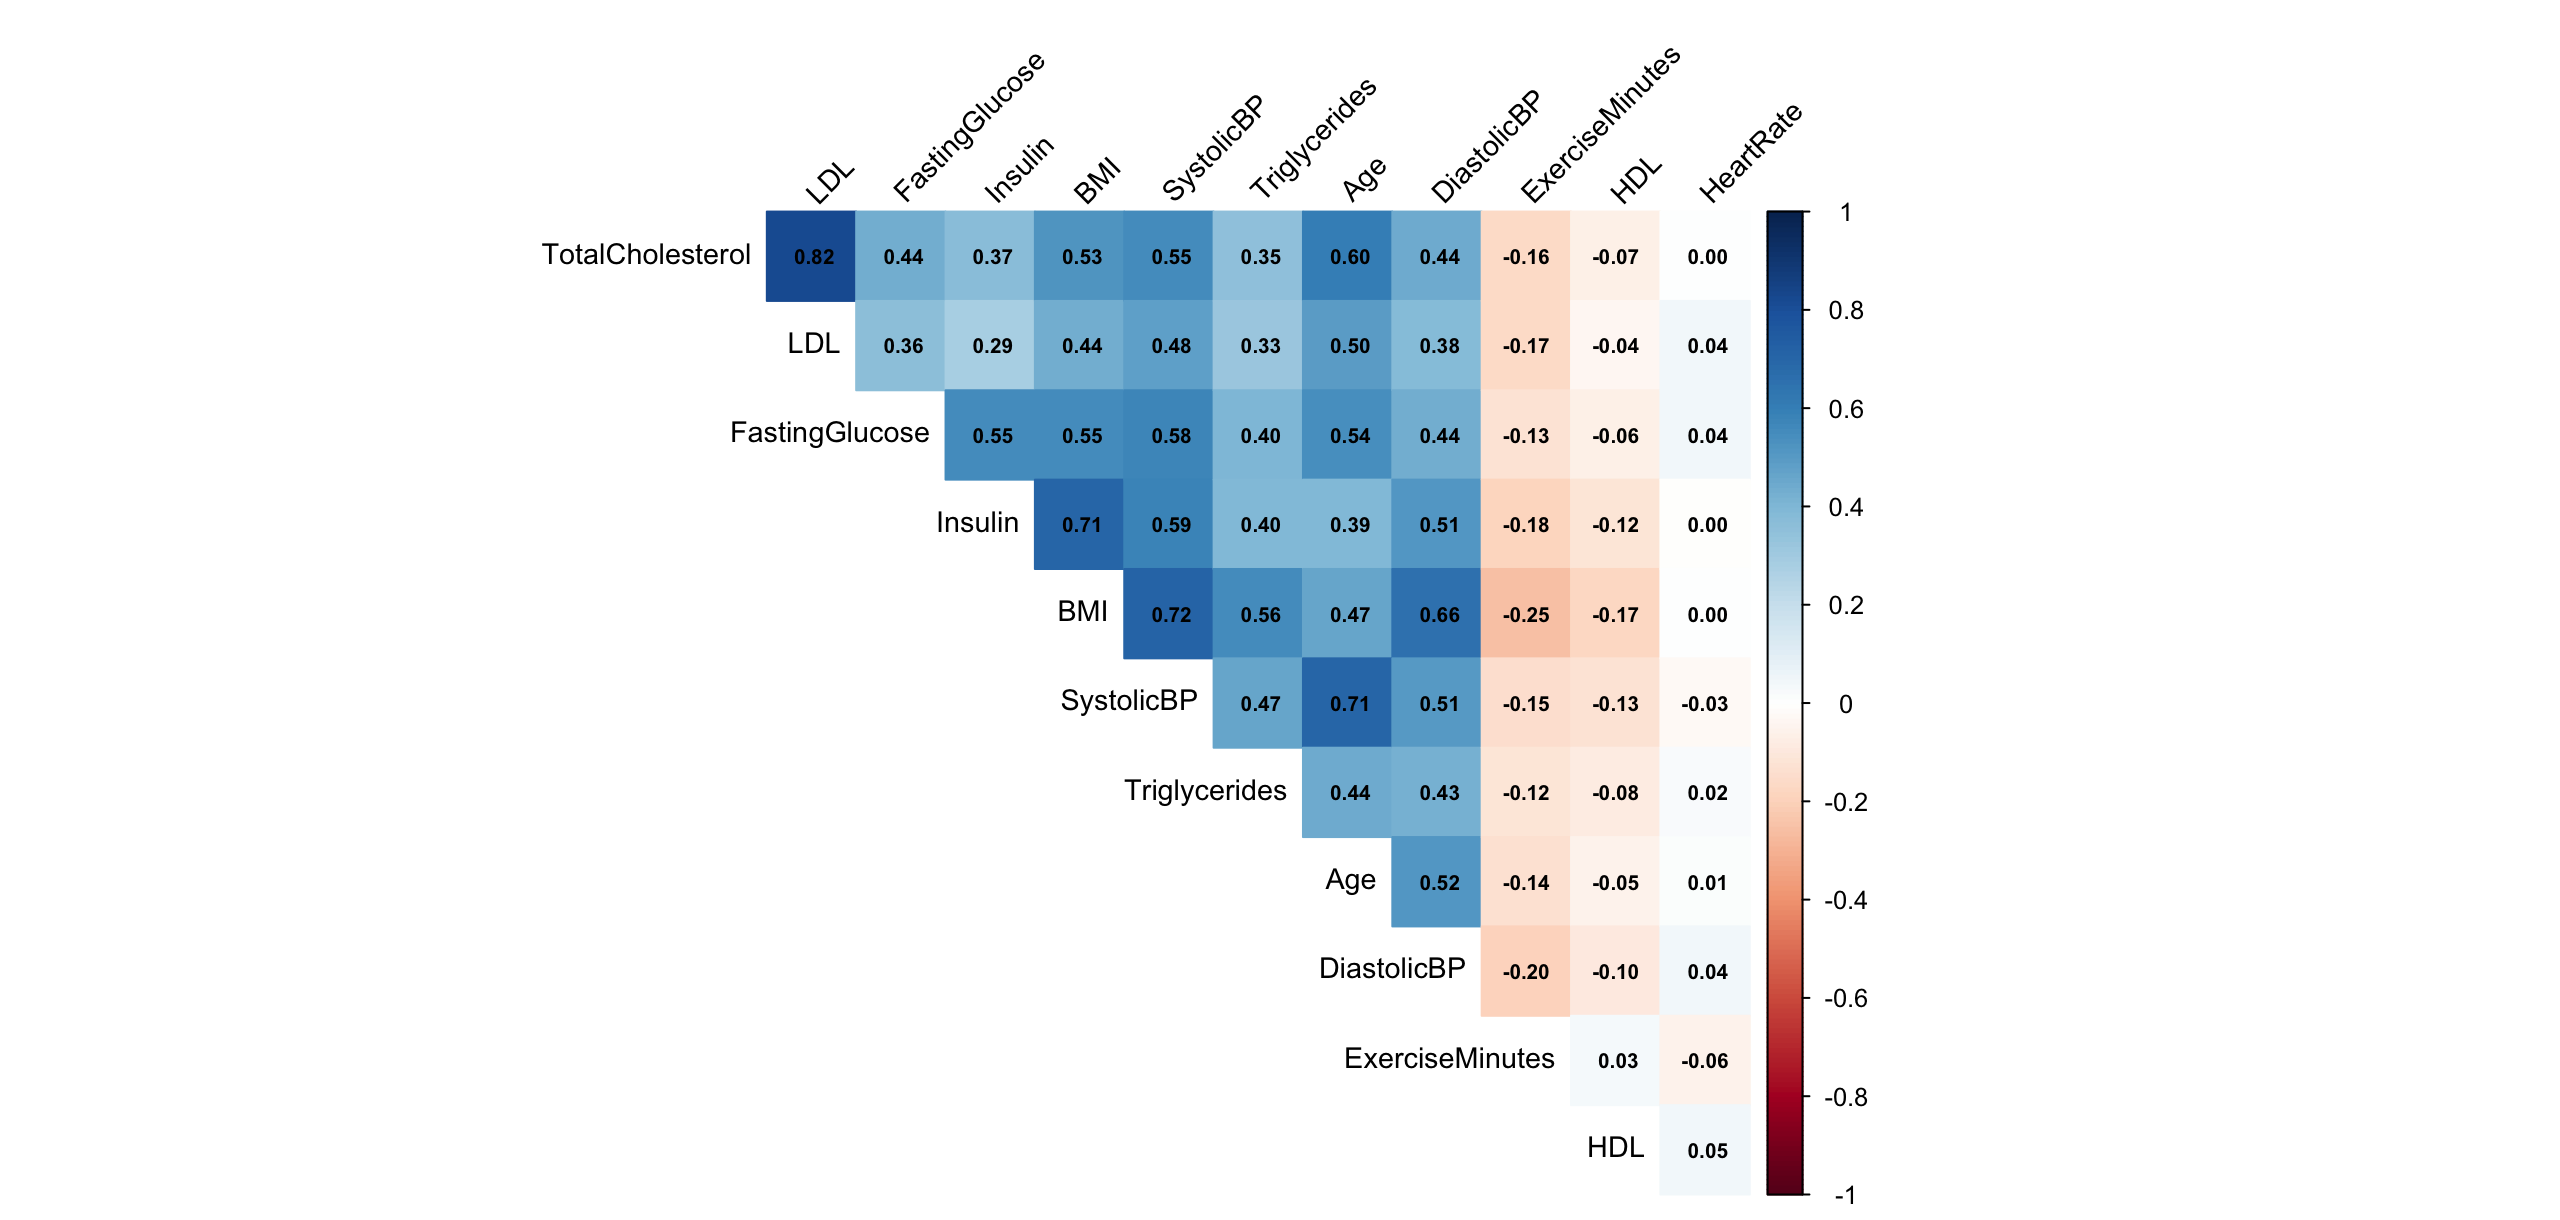
\includegraphics[width=0.8\textwidth]{assets/figures/heat.png}
\end{center}

\end{frame}




\begin{frame}{Correlation Heatmap}

\small

\begin{columns}[T]

% =====================================================
% LEFT COLUMN
% =====================================================

\column{0.42\textwidth}

\begin{itemize}

\item
A \textbf{heatmap} provides a visual summary of pairwise correlations between variables.

\vspace{0.25cm}

\item
Each cell shows the correlation coefficient
\[
r(X,Y)
\]
between two variables.

\vspace{0.25cm}

\item
Interpretation:

\begin{itemize}

\item
\textcolor{blue}{Blue}:
positive correlation.

\item
\textcolor{red}{Red}:
negative correlation.

\item
White/light colors:
weak or near-zero correlation.

\end{itemize}


\item
The closer $|\operatorname{Corr}(X,Y)|$ is to $1$, the stronger the linear relationship.

\end{itemize}

% =====================================================
% RIGHT COLUMN
% =====================================================

\column{0.58\textwidth}

\begin{center}
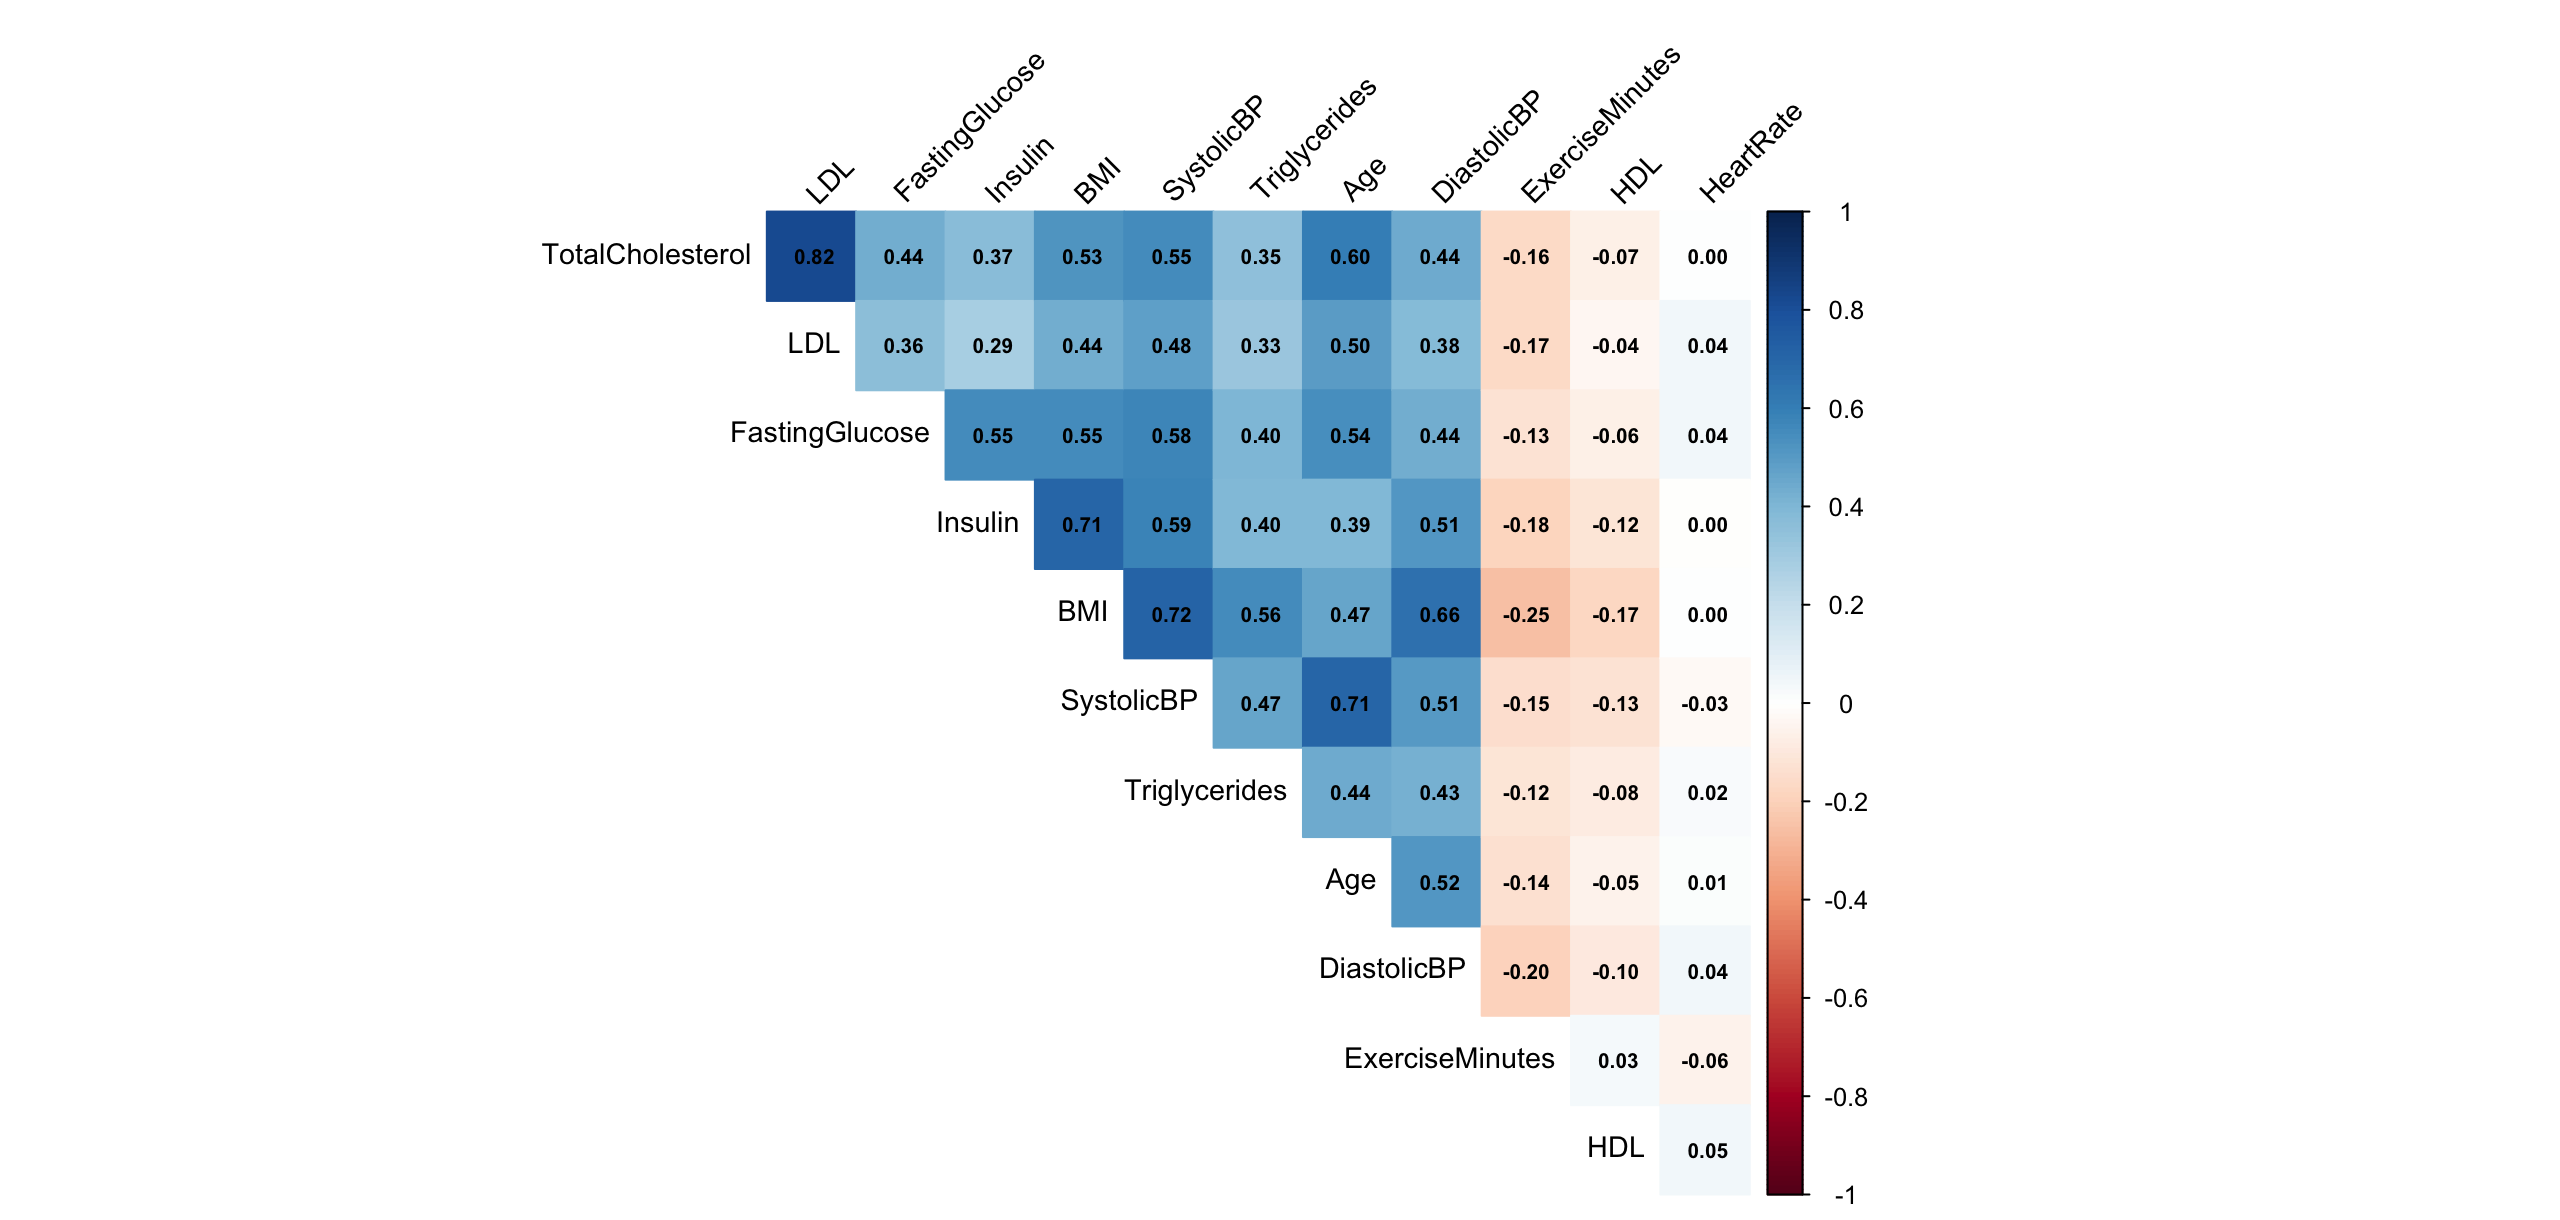
\includegraphics[
width=1.3\textwidth
]{assets/figures/heat.png}
\end{center}

\end{columns}

\end{frame}








\lecturepart{Multinomial Distribution}
\begin{frame}{Multinomial Distribution (generalization of Binomial Distribution)}

\textbf{In the Binomial setting}, each trial has two possible outcomes:
\[
o_1:\text{Success}
\qquad\text{or}\qquad
o_2: \text{Failure},
\]
with probabilities
\[
p_1 = p,\ \ 
p_2 = 1-p, \qquad where \qquad p_1 + p_2 =1
\]
After $n $ independent trials,
$$
X_1 :=X \qquad and \qquad X_2:= n-X
$$
count the number of trials resulting in category $o_1$: Success and $o_2$: Failure, respectively. Note that $X_1 + X_2 = X+ n-X=n$

\vspace{2mm}
\hrule
\vspace{2mm}

\textbf{In the multinomial setting}, each trial can result in one of $k$ (instead of 2) possible categories
\[
o_1,\dots,o_k,
\]
with probabilities
\[
p_1,\dots,p_k, \qquad where \qquad p_1 + \cdots + p_k=1
\]

After $n$ independent trials, 
\[
X_1,\dots X_k
\]
count the number of trials resulting in category $o_1,\dots, o_k$. Note that $X_1 + \dots +X_k=n$, since each trial results in exactly one category.

\end{frame}

\begin{frame}{Multinomial PMF}

\begin{keybox}{Definition}
If $(X_1,\dots,X_k)$ counts the numbers of occurrences of the $k$ categories in $n$ independent trials, then
\[
\boxed{
(X_1,\dots,X_k)
\sim
\operatorname{Mult}(n,p_1,\dots,p_k).
}
\]
\end{keybox}
\[
\boxed{
\Prob(X_1=x_1,\dots,X_k=x_k)
=
\frac{
n!
}{
x_1!\cdots x_k!
}
p_1^{x_1}\cdots p_k^{x_k},
}
\]

subject to:
\[
x_1+\cdots+x_k=n.
\]



\textbf{Note}. The Multinomial distribution is a multivariate distribution $k-dimensional$, while the Binomial is a univariable distribution $1-dimensional$. A multivariate random variable is also called a \textit{random vector}.
\vspace{1mm}
\textbf{Note}. It can be shown using the Multinomial Theorem (an extension of the Binomial Theorem) that the Multinomial PMF sums up to 1. Click \href{https://en.wikipedia.org/wiki/Multinomial_theorem}{here} to see the Multinomial Theorem in Wikipedia.

\end{frame}














%========================================================
\begin{frame}{Basic Properties of the Multinomial Distribution}

\begin{theorem}
Suppose
\[
(X_1,\dots,X_k)
\sim
\operatorname{Mult}(n,p_1,\dots,p_k),
\qquad
\sum_{i=1}^k p_i=1.
\]
Then,
\begin{enumerate}
    \item For every $i$,
    \[
    X_i\sim \operatorname{Bin}(n,p_i).
    \]

    \item More generally, if $A_1,\dots,A_r$ are disjoint subsets of $\{1,\dots,k\}$ and
    \[
    Y_j=\sum_{i\in A_j}X_i,
    \qquad
    q_j=\sum_{i\in A_j}p_i,
    \]
    then
    \[
    \left(
    Y_1,\dots,Y_r,\,
    n-\sum_{j=1}^rY_j
    \right)
    \sim
    \operatorname{Mult}
    \left(
    n,\,
    q_1,\dots,q_r,\,
    1-\sum_{j=1}^rq_j
    \right).
    \]
\end{enumerate}

\end{theorem}

\end{frame}

%========================================================
\begin{frame}{Multinomial Distribution: Trial Representation}

A multinomial experiment consists of $n$ independent trials.

For trial $\ell=1,\dots,n$, define
\[
I_{\ell i}
=
\begin{cases}
1, & \text{if trial $\ell$ results in category $i$},\\
0, & \text{otherwise}.
\end{cases}
\]

Then
\[
X_i=\sum_{\ell=1}^n I_{\ell i}.
\]

For every fixed $i$,
\[
I_{1i},\dots,I_{ni}
\overset{\text{i.i.d.}}{\sim}
\operatorname{Bernoulli}(p_i).
\]

Therefore,
\[
X_i
=
\sum_{\ell=1}^n I_{\ell i}
\sim
\operatorname{Bin}(n,p_i).
\]

Thus every individual component of a multinomial vector has a
binomial marginal distribution.

\end{frame}

%========================================================
\begin{frame}{Proof of the Grouping Property}

Let $A_1,\dots,A_r$ be disjoint subsets of $\{1,\dots,k\}$, and define $Y_j=\sum_{i\in A_j}X_i.$ For each trial $\ell$, define
\[
J_{\ell j}
=
\sum_{i\in A_j} I_{\ell i}.
\]

Since the sets $A_j$ are disjoint, $J_{\ell j}=1$ exactly when
trial $\ell$ falls into one of the categories in $A_j$.

Hence
\[
P(J_{\ell j}=1)
=
\sum_{i\in A_j}p_i
=
q_j.
\]

The remaining categories have probability
\[
1-\sum_{j=1}^r q_j.
\]

Therefore each trial can be viewed as having the new categories $A_1,\dots,A_r,\text{ remainder},
$ with probabilities
\[
q_1,\dots,q_r,\,
1-\sum_{j=1}^rq_j.
\]

Since the $n$ trials are independent,
\[
{
\left(
Y_1,\dots,Y_r,\,
n-\sum_{j=1}^rY_j
\right)
\sim
\operatorname{Mult}
\left(
n,q_1,\dots,q_r,
1-\sum_{j=1}^rq_j
\right).
}
\]

\end{frame}

%========================================================
\begin{frame}{Subvectors of a Multinomial Vector}

A useful special case is obtained by selecting some of the original
coordinates.

Suppose
\[
1\le i_1<\cdots<i_r\le k
\]
and define
\[
X_{\mathrm{rest}}
=
n-\sum_{j=1}^r X_{i_j}.
\]

Then
\[
\boxed{
\left(
X_{i_1},\dots,X_{i_r},X_{\mathrm{rest}}
\right)
\sim
\operatorname{Mult}
\left(
n,
p_{i_1},\dots,p_{i_r},
1-\sum_{j=1}^r p_{i_j}
\right).
}
\]

Thus a selected subvector is multinomial once all omitted categories
are combined into one ``remainder'' category.

In particular, for $i\neq j$,
\[
\boxed{
(X_i,X_j,n-X_i-X_j)
\sim
\operatorname{Mult}
(n,p_i,p_j,1-p_i-p_j).
}
\]

\end{frame}

%========================================================
\begin{frame}{Combining Categories}

The grouping property also shows that multinomial categories may be
combined.

For example, if
\[
(X_1,X_2,X_3,X_4)
\sim
\operatorname{Mult}(n,p_1,p_2,p_3,p_4),
\]
then $X_1+X_2$ counts trials falling in either category $1$ or category $2$. Therefore,
\[
\boxed{
X_1+X_2
\sim
\operatorname{Bin}(n,p_1+p_2).
}
\]

More generally, for any
\[
A\subseteq\{1,\dots,k\},
\]
\[
\boxed{
\sum_{i\in A}X_i
\sim
\operatorname{Bin}
\left(
n,\sum_{i\in A}p_i
\right).
}
\]

This follows by treating all categories in $A$ as one category and
all categories outside $A$ as another.

\end{frame}

%========================================================
\begin{frame}{Corollary: Means and Variances}

\begin{corollary}
If
\[
(X_1,\dots,X_k)
\sim
\operatorname{Mult}(n,p_1,\dots,p_k),
\]
then, for every $i$,
\[
E(X_i)=np_i
\]
and
\[
\Var(X_i)=np_i(1-p_i).
\]
\end{corollary}

\begin{proof}
Since
\[
X_i\sim\operatorname{Bin}(n,p_i),
\]
the usual formulas for a binomial random variable immediately give
\[
{E(X_i)=np_i}
\]
and
\[
{\Var(X_i)=np_i(1-p_i)}.
\]
\end{proof}

\end{frame}

%========================================================
\begin{frame}{Covariance Between Multinomial Counts}

For $i\neq j$, use the trial representation
\[
X_i=\sum_{\ell=1}^n I_{\ell i},
\qquad
X_j=\sum_{\ell=1}^n I_{\ell j}.
\]

Therefore,
\[
\Cov(X_i,X_j)
=
\sum_{\ell=1}^n\sum_{m=1}^n
\Cov(I_{\ell i},I_{mj}).
\]

If $\ell\neq m$, the trials are independent, so
\[
\Cov(I_{\ell i},I_{mj})=0.
\]

Hence
\[
\Cov(X_i,X_j)
=
\sum_{\ell=1}^n
\Cov(I_{\ell i},I_{\ell j}).
\]

\end{frame}

%========================================================
\begin{frame}{Covariance Between Multinomial Counts}

For the same trial $\ell$, categories $i$ and $j$ cannot occur
simultaneously when $i\neq j$. Thus
\[
I_{\ell i}I_{\ell j}=0,
\]
so
\[
E(I_{\ell i}I_{\ell j})=0.
\]

Also,
\[
E(I_{\ell i})=p_i,
\qquad
E(I_{\ell j})=p_j.
\]

Therefore,
\begin{align*}
\Cov(I_{\ell i},I_{\ell j})
&=
E(I_{\ell i}I_{\ell j})
-
E(I_{\ell i})E(I_{\ell j})\\
&=
0-p_ip_j\\
&=
-p_ip_j.
\end{align*}

Thus
\[
\boxed{
\Cov(X_i,X_j)
=
-np_ip_j,
\qquad i\neq j.
}
\]

\end{frame}

%========================================================
\begin{frame}{Why Is the Covariance Negative?}

For $i\neq j$,
\[
\Cov(X_i,X_j)=-np_ip_j<0
\]
whenever $p_i,p_j>0$.

This has a natural interpretation.

The total number of trials is fixed:
\[
X_1+\cdots+X_k=n.
\]

Thus, if more observations fall into category $i$, fewer observations
are available to fall into the other categories.

So the multinomial counts are generally \emph{not independent}.

For example,
\[
X_i\uparrow
\quad\Longrightarrow\quad
\text{less room for }X_j\uparrow.
\]

This competition for a fixed total produces the negative covariance.

\end{frame}

%========================================================
\begin{frame}{Mean Vector and Covariance Matrix}

Let
\[
X=
\begin{pmatrix}
X_1\\
\vdots\\
X_k
\end{pmatrix},
\qquad
p=
\begin{pmatrix}
p_1\\
\vdots\\
p_k
\end{pmatrix}.
\]

Then
\[
\boxed{
E(X)=np.
}
\]

The covariance matrix has diagonal entries
\[
np_i(1-p_i)
\]
and off-diagonal entries
\[
-np_ip_j.
\]

Therefore,
\[
\boxed{
\Cov(X)
=
n\left[
\operatorname{diag}(p)-pp^{T}
\right].
}
\]

\end{frame}





















\lecturepart{Multivariate Normal Distribution}


\begin{frame}{Bivariate Normal Distribution}

\begin{keybox}{Big Picture}
The bivariate normal distribution is the two-dimensional version of the normal distribution.

It describes two continuous random variables $X$ and $Y$ whose joint density has a bell-shaped surface over the $xy$-plane.
\end{keybox}

\vspace{0.25cm}

A bivariate normal distribution is determined by five parameters:
\[
\mu_X,\quad \mu_Y,\quad \sigma_X^2,\quad \sigma_Y^2,\quad \rho.
\]

Here,
\[
\rho=\operatorname{Corr}(X,Y)
\]
controls the strength and direction of the linear relationship between $X$ and $Y$.

\vspace{0.3cm}

\centering
\href{https://armanjg.github.io/MATH-394-Probability-1-v2/Figures/bivariate.html}{\beamergotobutton{Open interactive bivariate normal visualization}}
Click this link for interactive bivariate normal visualization.

\end{frame}




\begin{frame}{Bivariate Normal Distribution: Density}

\begin{keybox}{Definition}
We say
\[
(X,Y)
\sim
N_2
\left(
\begin{pmatrix}
\mu_X\\
\mu_Y
\end{pmatrix},
\begin{pmatrix}
\sigma_X^2 & \rho\sigma_X\sigma_Y\\
\rho\sigma_X\sigma_Y & \sigma_Y^2
\end{pmatrix}
\right)
\]
if the joint density of $(X,Y)$ is
\[
\begin{aligned}
f_{X,Y}(x,y)
&=
\frac{1}{2\pi \sigma_X\sigma_Y\sqrt{1-\rho^2}}
\\[0.15cm]
&\quad \times
\exp\left\{
-\frac{1}{2(1-\rho^2)}
\left[
\left(\frac{x-\mu_X}{\sigma_X}\right)^2
-2\rho
\left(\frac{x-\mu_X}{\sigma_X}\right)
\left(\frac{y-\mu_Y}{\sigma_Y}\right)
+
\left(\frac{y-\mu_Y}{\sigma_Y}\right)^2
\right]
\right\}.
\end{aligned}
\]
\end{keybox}

where $\sigma_X>0$, $\sigma_Y>0$, and $-1<\rho<1$.

\end{frame}



\begin{frame}{Bivariate Normal Distribution: Main Properties}

If
\[
(X,Y)
\sim
N_2
\left(
\begin{pmatrix}
\mu_X\\
\mu_Y
\end{pmatrix},
\begin{pmatrix}
\sigma_X^2 & \rho\sigma_X\sigma_Y\\
\rho\sigma_X\sigma_Y & \sigma_Y^2
\end{pmatrix}
\right),
\]
then:

\vspace{0.2cm}

\begin{itemize}
    \item The means are
    \[
    \mathbb{E}(X)=\mu_X,
    \qquad
    \mathbb{E}(Y)=\mu_Y.
    \]

    \item The variances are
    \[
    \operatorname{Var}(X)=\sigma_X^2,
    \qquad
    \operatorname{Var}(Y)=\sigma_Y^2.
    \]

    \item The covariance is
    \[
    \operatorname{Cov}(X,Y)=\rho\sigma_X\sigma_Y.
    \]

    \item Therefore,
    \[
    \operatorname{Corr}(X,Y)=\rho.
    \]
\end{itemize}

\end{frame}





\begin{frame}{Marginal Distributions}

A beautiful property of the bivariate normal distribution is that the marginal distributions are normal.

\begin{keybox}{Marginals}
If
\[
(X,Y)
\sim
N_2
\left(
\begin{pmatrix}
\mu_X\\
\mu_Y
\end{pmatrix},
\begin{pmatrix}
\sigma_X^2 & \rho\sigma_X\sigma_Y\\
\rho\sigma_X\sigma_Y & \sigma_Y^2
\end{pmatrix}
\right),
\]
then
\[
\boxed{
X\sim N(\mu_X,\sigma_X^2)
}
\]
and
\[
\boxed{
Y\sim N(\mu_Y,\sigma_Y^2).
}
\]
\end{keybox}

\vspace{0.25cm}

So the joint distribution is bivariate normal, but each marginal variable individually is ordinary normal.

\end{frame}





\begin{frame}{Conditional Distributions}

Another beautiful property is that the conditional distributions are also normal.

\begin{keybox}{Conditionals}
If
\[
(X,Y)
\]
is bivariate normal, then
\[
\boxed{
X\mid Y=y
\sim
N
\left(
\mu_X
+
\rho\frac{\sigma_X}{\sigma_Y}(y-\mu_Y),
\;
\sigma_X^2(1-\rho^2)
\right)
}
\]

and

\[
\boxed{
Y\mid X=x
\sim
N
\left(
\mu_Y
+
\rho\frac{\sigma_Y}{\sigma_X}(x-\mu_X),
\;
\sigma_Y^2(1-\rho^2)
\right).
}
\]
\end{keybox}

\vspace{0.2cm}

The conditional mean is linear in the observed value.

\end{frame}




\begin{frame}{Independence and Zero Correlation}

For general random variables,
\[
\operatorname{Corr}(X,Y)=0
\]
does not necessarily imply independence.

\vspace{0.25cm}

But for the bivariate normal distribution, it does.

\begin{keybox}{Important Gaussian Property}
If $(X,Y)$ is bivariate normal, then
\[
\boxed{
X \text{ and } Y \quad independent
\quad\Longleftrightarrow\quad
\rho=0.
}
\]
\end{keybox}

\vspace{0.25cm}

When $\rho=0$, the joint density factors:
\[
f_{X,Y}(x,y)
=
f_X(x)f_Y(y).
\]

So in the bivariate normal case,
\[
\text{uncorrelated}
\quad\Longleftrightarrow\quad
\text{independent}.
\]

\end{frame}



















